\documentclass{article}

% Configuración de idioma en español
\usepackage[spanish]{babel}
\usepackage[utf8]{inputenc}
\usepackage{booktabs}
\usepackage{array}
\usepackage{tikz}
\usetikzlibrary{babel, arrows.meta, positioning, shapes.geometric, calc}

% Configuración de página y márgenes
\usepackage[letterpaper,top=2cm,bottom=2cm,left=3cm,right=3cm,marginparwidth=1.75cm]{geometry}

% Paquetes útiles
\usepackage{amsmath}
\usepackage{graphicx}
\usepackage{float} % [H] fija cada figura donde está en el código
\usepackage[colorlinks=true, allcolors=blue]{hyperref}

\title{AnyDrums VR}
\author{Gonzalez Kremer, Mauricio Gabriel \and Rojas Cruz, José Alvaro \and Llerena Silva, Nicolás Alejandro}

\begin{document}
\maketitle

\section{Antecedentes}

El aprendizaje y la práctica de la batería acústica tradicional presentan importantes barreras de entrada en el mundo físico: el elevado costo del instrumento, el amplio espacio requerido para su instalación y el alto nivel de ruido que genera, lo cual limita su uso en departamentos o entornos compartidos. A partir de las actividades exploradas durante los laboratorios del curso sobre diseño de entornos virtuales, locomoción e interacción física tridimensional en Unity, este proyecto aborda dicho espacio del problema mediante el desarrollo de un simulador de batería en Realidad Virtual (VR). El sistema contempla un conjunto completo conformado por \textit{hi-hat}, platos (\textit{ride} y \textit{crash}), \textit{Tom 1}, \textit{Tom 2}, \textit{tom base}, caja y bombo, permitiendo al usuario tocar en un ambiente inmersivo lo más cercano posible a la realidad al producir sonidos según la zona de impacto y la fuerza aplicada con las baquetas virtuales \cite{batery_asset, samples}.

Diversos trabajos relacionados han demostrado la viabilidad de la Realidad Virtual para superar las limitaciones espaciales y acústicas de la percusión tradicional. En el ámbito académico, investigaciones como \textit{VRumset} de Glisson (2023) evidencian que los entornos inmersivos permiten enseñar y practicar rudimentos de batería sin necesidad de contar con el espacio físico ni generar contaminación sonora, destacando a su vez retos técnicos clave en el seguimiento de colisiones a alta velocidad \cite{glisson2023}. De manera complementaria, aplicaciones comerciales de referencia como \textit{Paradiddle} han establecido estándares en la simulación de percusión en VR al incorporar variaciones acústicas dependientes de la velocidad de golpeo y la posición de impacto sin requerir hardware musical físico adicional \cite{paradiddle}. Tomando como base estos antecedentes, nuestra propuesta se enfoca en optimizar la fidelidad física y auditiva mediante detección continua de colisiones y modulación dinámica del sonido en tiempo real.

\section{Requisitos de diseño y persona}

\subsection{Requisitos funcionales}
A partir del análisis de las necesidades de los usuarios y la mecánica real de percusión, se definieron los siguientes requisitos funcionales junto con su justificación de diseño:

\begin{itemize}
    \item \textbf{RF1 - Selección de modalidad de batería (Acústica y Electrónica) - MUST HAVE:} Al iniciar la aplicación, el menú principal debe permitir al usuario elegir entre un kit acústico y uno electrónico, cargando su respectivo banco de \textit{samples}. \textit{Importancia:} Permite adaptarse a distintos géneros musicales y preferencias auditivas del usuario sin necesidad de cambiar de entorno.
    \item \textbf{RF2 - Interacción física mediante baquetas virtuales - MUST HAVE:} El usuario debe poder sujetar y mover dos baquetas virtuales para golpear el \textit{hi-hat}, los platos (\textit{ride} y \textit{crash}), el \textit{Tom 1}, el \textit{Tom 2}, el \textit{tom base} y la caja. Los dos pedales, que en una batería real se accionan con los pies, pasan a los gatillos porque el Meta Quest 2 no hace seguimiento de los pies: el gatillo del mando derecho toca el bombo y el del mando izquierdo funciona como el pedal del \textit{hi-hat} (presionado lo cierra y suelto lo deja abierto). \textit{Importancia:} Constituye la acción nuclear (\textit{core loop}) de la simulación; sin un mapeo directo de las manos hacia las baquetas, se pierde la transferencia de habilidad motora.
    \item \textbf{RF3 - Modulación acústica según fuerza y zona de impacto - MUST HAVE:} El sistema debe calcular la velocidad del golpe y la distancia radial desde el centro del tambor ($0.0$ en el centro a $1.0$ en el borde) para ajustar dinámicamente el volumen y el tono (\texttt{AudioSource.pitch}) del sonido reproducido. En el bombo, como no hay zona de impacto, la fuerza se obtiene de la rapidez con que se presiona el gatillo. En el \textit{hi-hat}, además, el sonido depende de qué tan presionado esté el gatillo izquierdo al momento del golpe (abierto, semiabierto o cerrado). \textit{Importancia:} En una batería real, el timbre varía drásticamente según dónde y qué tan fuerte se golpee; este requisito es indispensable para alcanzar la fidelidad buscada.
    \item \textbf{RF4 - Control y ajuste de volumen:} La interfaz debe ofrecer un control accesible para regular el volumen general del simulador. \textit{Importancia:} Protege la comodidad auditiva del usuario en sesiones prolongadas con auriculares de VR.
    \item \textbf{RF5 - Locomoción por teletransportación:} El usuario debe poder desplazarse en el entorno mediante teletransportación para ubicarse frente a la batería. \textit{Importancia:} Evita la incomodidad de realizar ajustes milimétricos con el \textit{joystick} y reduce el riesgo de cinetosis (\textit{motion sickness}).
\end{itemize}

\subsection{Requisitos no funcionales}
Para garantizar la usabilidad y la inmersión del simulador en VR, se establecieron los siguientes requisitos no funcionales:

\begin{itemize}
    \item \textbf{RNF1 - Prevención de tunelamiento (\textit{anti-tunneling}) en colisiones rápidas:} Las baquetas nunca deben atravesar las mallas de los tambores, incluso durante redobles o movimientos de alta velocidad, empleando \textit{Continuous Collision Detection} (CCD) y \texttt{Physics.SphereCast}. \textit{Importancia:} En canciones rápidas la velocidad de los controles supera el muestreo discreto por frame; si la baqueta atraviesa el tambor sin sonar, se rompe inmediatamente el sentido de presencia.
    \item \textbf{RNF2 - Estabilidad en el cálculo de velocidad de impacto:} La velocidad de golpeo debe estimarse mediante un buffer manual de los últimos $3$ a $5$ frames en lugar de depender únicamente del \texttt{Rigidbody}. \textit{Importancia:} Compensa las fluctuaciones o pérdidas momentáneas del seguimiento óptico de los mandos VR, garantizando una respuesta sonora consistente.
    \item \textbf{RNF3 - Baja latencia auditiva y alta tasa de refresco:} El retardo entre la colisión física y la emisión del sonido debe ser imperceptible (idealmente $<20\text{ ms}$) manteniendo una tasa estable de $72$ cuadros por segundo, que es la frecuencia base del Meta Quest 2. \textit{Importancia:} La ejecución rítmica depende de la retroalimentación auditiva inmediata; cualquier desfase impide mantener el tempo musical.
    \item \textbf{RNF4 - Fidelidad de escala espacial (1:1):} Las dimensiones y disposición de las piezas de la batería deben corresponder al tamaño de ejemplares reales. \textit{Importancia:} Permite que la memoria muscular del usuario coincida con las distancias físicas reales de una batería.
\end{itemize}

\subsection{Audiencia}
Nuestro público objetivo está conformado por personas que poseen un dispositivo de Realidad Virtual (VR) y tienen interés en interactuar con instrumentos musicales de percusión, específicamente una batería acústica o electrónica, ya sea para iniciarse en el instrumento o para practicar en lugares donde no podrían instalar una batería real por limitaciones de espacio, transporte o ruido.

Dentro de esta audiencia se identifican dos perfiles principales (\textit{Personas}) y sus respectivos roles dentro de la aplicación:
\begin{itemize}
    \item \textbf{Practicante / Músico aficionado (Rol: Intérprete activo):} Usuarios con conocimientos básicos o intermedios de ritmo que buscan ensayar libremente, mantener su memoria muscular y experimentar con matices dinámicos (fuerza y zona de golpeo) sin generar molestias acústicas en su entorno doméstico.
    \item \textbf{Entusiasta curioso de VR (Rol: Explorador musical):} Usuarios propietarios de visores VR sin formación musical previa ni acceso a una batería física, cuyo propósito es probar el instrumento de forma accesible, intuitiva y lúdica por primera vez.
\end{itemize}

\subsection{Especificación final de persona}
A continuación, se presenta la especificación detallada del usuario arquetípico principal (\textit{User Persona}) que guía las decisiones de diseño del simulador:

\begin{itemize}
    \item \textbf{Nombre y perfil:} Diego Morales (21 años, estudiante universitario residente en un departamento multifamiliar).
    \item \textbf{Contexto tecnológico y musical:} Cuenta con un visor de Realidad Virtual autónomo en su habitación. Le apasiona la música rock y electrónica; aprendió los conceptos básicos de batería en el pasado, pero no posee un instrumento propio.
    \item \textbf{Objetivos:}
    \begin{enumerate}
        \item Practicar ritmos y coordinar el movimiento de brazos en un entorno con escala real (1:1).
        \item Percibir una respuesta auditiva realista que distinga entre golpes suaves y fuertes, así como entre el centro y el borde de cada tambor o plato.
        \item Alternar fácilmente entre el timbre de una batería acústica y una electrónica según el estilo musical que desee tocar.
    \end{enumerate}
    \item \textbf{Frustraciones y puntos de dolor:}
    \begin{enumerate}
        \item No puede adquirir ni instalar una batería física en su departamento debido al elevado costo, la falta de espacio y las quejas de los vecinos por el ruido.
        \item En otros juegos o simuladores básicos, siente que las baquetas atraviesan los objetos cuando toca rápido o que el sonido es plano y artificial (suena igual sin importar la fuerza del golpe).
        \item Le incomoda el mareo por movimiento (\textit{motion sickness}) cuando debe desplazarse con \textit{joystick} continuo para acomodarse frente a objetos virtuales.
    \end{enumerate}
\end{itemize}

\subsection{Objetivo de la experiencia}
El objetivo principal de la experiencia es proporcionar al usuario un entorno inmersivo, accesible y de alta fidelidad física y acústica en Realidad Virtual donde pueda tocar una batería completa (compuesta por \textit{hi-hat}, platos \textit{ride} y \textit{crash}, \textit{Tom 1} y \textit{2}, \textit{tom base}, caja y bombo) sintiendo una respuesta inmediata y natural. Se busca que el usuario logre expresividad musical real mediante la variación de fuerza y zona de impacto con las baquetas, eliminando por completo las barreras espaciales y de contaminación sonora del mundo físico.

\subsection{Narrativa de la aplicación}
La aplicación sitúa al usuario en un estudio de práctica virtual privado y libre de distracciones, diseñado para que pueda concentrarse exclusivamente en la ejecución musical. Al ingresar a la experiencia, el usuario es recibido por un panel de configuración inicial donde define la identidad sonora de su sesión: puede optar por la calidez orgánica de una batería acústica o la versatilidad moderna de una batería electrónica, además de calibrar el volumen general a su nivel de confort. Una vez confirmada su elección, el usuario es posicionado frente al conjunto de percusión a escala real con un par de baquetas en sus manos virtuales, listo para desplazarse mediante teletransportación hasta su postura ideal e iniciar su interpretación libre.

\subsection{Arco de la historia}
El flujo de la experiencia del usuario a lo largo de una sesión sigue un arco estructurado en cinco etapas:

\begin{enumerate}
    \item \textbf{Exposición (Ingreso y configuración):} El usuario inicia la aplicación en VR y visualiza el menú principal. Allí selecciona entre la modalidad de batería acústica o electrónica y ajusta el nivel de volumen.
    \item \textbf{Incidente incitador (Encuentro con el instrumento):} El usuario aparece en el entorno junto a la batería seleccionada a escala real y toma el control de las baquetas virtuales.
    \item \textbf{Acción creciente (Acomodación y exploración sonora):} Utilizando el sistema de teletransportación, el usuario se ubica en la posición ergonómica perfecta frente al kit. Comienza a dar los primeros golpes de prueba en la caja, el \textit{hi-hat}, los \textit{toms} y los platos, descubriendo cómo el sonido cambia dinámicamente según la fuerza aplicada y qué tan cerca del centro o del borde impacta cada pieza.
    \item \textbf{Clímax (Interpretación fluida):} El usuario ejecuta ritmos continuos y redobles a alta velocidad con total inmersión; el sistema responde con precisión sin que las baquetas atraviesen las mallas (\textit{anti-tunneling}) y manteniendo una retroalimentación auditiva coherente en tiempo real.
    \item \textbf{Desenlace (Cierre de sesión):} Satisfecho con la práctica musical, el usuario puede regresar al menú para cambiar de tipo de batería (de acústica a electrónica o viceversa), reajustar el volumen o finalizar la sesión.
\end{enumerate}

\subsection{Métrica HEART}
Para evaluar cuantitativa y cualitativamente el éxito de la experiencia de usuario y la usabilidad del simulador, se emplea el framework \textbf{HEART} (\textit{Happiness, Engagement, Adoption, Retention, Task Success}), detallando los objetivos, señales y métricas específicas en el Cuadro \ref{tab:heart}:

\begin{table}[H]
\centering
\small
\renewcommand{\arraystretch}{1.4} % Da aire vertical entre filas
\begin{tabular}{@{} >{\bfseries}p{0.18\textwidth} >{\raggedright\arraybackslash}p{0.25\textwidth} >{\raggedright\arraybackslash}p{0.25\textwidth} >{\raggedright\arraybackslash}p{0.25\textwidth} @{}}
\toprule
Dimensión & \textbf{Objetivo (\textit{Goal})} & \textbf{Señal (\textit{Signal})} & \textbf{Métrica (\textit{Metric})} \\
\midrule
Happiness \newline \normalfont\footnotesize(Felicidad) &
Que el usuario perciba una alta fidelidad acústica/física y comodidad durante la sesión. &
Valoración positiva de la respuesta sonora y ausencia de fatiga o mareo en encuestas post-prueba. &
Puntaje promedio en cuestionario de satisfacción (escala Likert 1--5) y puntaje SUS (\textit{System Usability Scale}). \\
\addlinespace[0.4em]
Engagement \newline \normalfont\footnotesize(Compromiso) &
Fomentar la práctica activa y la exploración de todas las piezas del kit de batería. &
Interacción constante con los distintos tambores/platos y prolongación voluntaria de la sesión. &
Tiempo promedio de sesión activa (en minutos) y número total de golpes registrados por minuto. \\
\addlinespace[0.4em]
Adoption \newline \normalfont\footnotesize(Adopción) &
Lograr que los usuarios utilicen tanto la modalidad acústica como la electrónica y personalicen su entorno. &
Uso efectivo del menú inicial para alternar entre ambos kits de \textit{samples} y ajustar el volumen. &
Porcentaje de usuarios que prueban ambas configuraciones de batería durante su primera sesión. \\
\addlinespace[0.4em]
Retention \newline \normalfont\footnotesize(Retención) &
Motivar al usuario a volver a utilizar el simulador como herramienta habitual de práctica. &
Usuarios que reingresan a la aplicación en días posteriores o repiten rondas de práctica. &
Tasa de retorno de usuarios en sesiones de prueba subsecuentes y frecuencia de reintento. \\
\addlinespace[0.4em]
Task Success \newline \normalfont\footnotesize(Éxito de tarea) &
Garantizar una ejecución rítmica precisa, sin fallos de colisión y con rápido posicionamiento espacial. &
Golpes rápidos detectados correctamente sin atravesar el tambor y rápido acomodo frente al kit. &
Tasa de detección efectiva de colisiones rápidas ($>95\%$) y tiempo promedio en ubicarse mediante teletransportación. \\
\bottomrule
\end{tabular}
\caption{\label{tab:heart}Matriz de evaluación basada en el framework HEART para el simulador de batería en VR.}
\end{table}

\section{Framework de diseño}

El diseño de nuestra aplicación se fundamenta en un framework de interacción tridimensional directa y diseño visual centrado en el usuario, aplicando explícitamente conceptos fundamentales de Interacción Humano-Computador (IHC) y Realidad Virtual vistos en clase:

\begin{itemize}
    \item \textbf{\textit{Affordances} (Perceptibilidad) y \textit{Signifiers} (Indicadores):} Siguiendo los principios de diseño de Don Norman, el modelo 3D de la batería y las baquetas poseen \textit{affordances} físicas claras: su geometría y disposición espacial comunican de forma intuitiva que las baquetas están diseñadas para sujetarse y las superficies de los tambores y platos para ser golpeadas, sin requerir extensos tutoriales escritos.
    \item \textbf{Mapeo Natural (\textit{Natural Mapping}) y Escala 1:1:} Existe una correspondencia espacial directa entre el movimiento físico de las manos del usuario con los mandos VR y el desplazamiento de las baquetas virtuales en el entorno 3D. Al mantener las dimensiones reales del instrumento, se aprovecha la propiocepción del usuario. Las únicas excepciones son los pedales, porque el visor no rastrea los pies: el bombo pasa del pie derecho al gatillo derecho y el pedal del \textit{hi-hat}, del pie izquierdo al gatillo izquierdo. Mantuvimos el mismo lado del cuerpo que en una batería real para que la correspondencia sea fácil de recordar.
    \item \textbf{Retroalimentación (\textit{Feedback}) Multimodal Inmediata:} Toda acción del usuario genera una respuesta instantánea en el sistema. Al impactar un componente, la retroalimentación auditiva varía dinámicamente en volumen y tono (\textit{pitch}) según la fuerza y la distancia radial al centro del tambor, y el mando vibra brevemente con una intensidad proporcional a la fuerza del golpe, cerrando el ciclo de acción-evaluación en milisegundos.
    \item \textbf{Ley de Fitts y Ergonomía Espacial:} Tanto los botones del menú inicial como la disposición semicircular de los componentes de la batería (caja, \textit{hi-hat}, \textit{Tom 1}, \textit{Tom 2}, \textit{tom base}, bombo y platos \textit{ride} y \textit{crash}) se ubican a una distancia y tamaño óptimos respecto al punto de origen del usuario, minimizando el tiempo de desplazamiento balístico de los brazos y reduciendo la fatiga física.
    \item \textbf{Prevención de Cinetosis (\textit{Motion Sickness}):} Para el desplazamiento dentro del escenario se descarta el movimiento continuo por \textit{joystick}, que genera conflicto vestibular entre la vista y el oído interno, y se opta por locomoción mediante teletransportación discreta, permitiendo un encuadre rápido y cómodo frente al instrumento.
\end{itemize}

\section{Descripción del framework}

El flujo de interacción y la composición visual se articulan en dos espacios principales dentro de la experiencia:

En primer lugar, cuando el usuario ingresa a la aplicación, lo primero que visualiza es una interfaz de menú espacial (\textit{World-Space UI}) limpia y de alto contraste, situada a una distancia de lectura ergonómica. Inicialmente, este panel presenta dos opciones principales de configuración: una para seleccionar una \textbf{batería acústica} y otra para una \textbf{batería electrónica}. Cada modalidad carga su respectivo banco de \textit{samples} de sonido para transformar la respuesta tímbrica del instrumento \cite{samples}. Asimismo, en esta interfaz se otorga al usuario la capacidad de ajustar el volumen general mediante un control deslizable (\textit{slider}) según vea conveniente para su confort auditivo.

En segundo lugar, una vez confirmada la selección, el usuario aparece posicionado cerca de la batería de su elección dentro de un entorno virtual despejado que dirige el foco visual hacia el instrumento. El diseño visual emplea texturas diferenciadas para los parches de los tambores, el metal de los platos y la madera de las baquetas \cite{batery_asset}, facilitando la distinción visual periférica mientras el usuario ejecuta ritmos y utiliza las baquetas virtuales para interactuar libremente con todo el equipo.

\section{Plan de diseño}

A continuación, se detallan los tres ejes fundamentales que estructuran nuestro plan de diseño en Realidad Virtual:

\subsection{¿Qué pueden lograr tus usuarios? ¿Qué pueden hacer?}
Los usuarios pueden experimentar la práctica y ejecución libre de percusión en un entorno virtual sin las restricciones físicas de espacio o ruido de una batería real. Concretamente, dentro de la aplicación pueden:
\begin{enumerate}
    \item Seleccionar en el menú inicial entre un kit de batería acústica o electrónica y calibrar el volumen del entorno.
    \item Desplazarse por el escenario mediante teletransportación para acomodarse en su postura ideal frente al instrumento sin depender de toques imprecisos al \textit{joystick}.
    \item Empuñar las baquetas virtuales y golpear el \textit{hi-hat}, los platos \textit{ride} y \textit{crash}, el \textit{Tom 1} y \textit{2}, el \textit{tom base} y la caja; tocar el bombo con el gatillo del mando derecho y abrir o cerrar el \textit{hi-hat} con el gatillo del mando izquierdo.
    \item Producir matices musicales expresivos modulando la fuerza de sus golpes (que altera el volumen y el \texttt{pitch}) y variando la zona de impacto sobre el tambor (desde el centro en $0.0$ hasta el borde en $1.0$).
\end{enumerate}

\subsection{¿Cuáles son los límites técnicos o de su experiencia?}
En cuanto a los límites técnicos, el principal desafío radica en la tasa de refresco y la detección de colisiones entre frames (\textit{frame rate} y muestreo físico). Como sabemos, la ejecución de la batería en muchas canciones exige una interacción sumamente rápida y fuerte; si una baqueta se mueve a gran velocidad entre dos frames consecutivos, el motor de físicas estándar podría no registrar el impacto o permitir que las mallas de las baquetas atraviesen los tambores (\textit{tunneling}), algo que nunca debe ocurrir. Del mismo modo, el seguimiento óptico (\textit{tracking}) de los controles VR no es $100\%$ confiable ante movimientos bruscos, lo que obliga a implementar un cálculo manual de velocidad con un buffer de $3$ a $5$ frames junto con \textit{Continuous Collision Detection} (CCD) y \texttt{Physics.SphereCast}.

En cuanto a los límites de la experiencia, existe la ausencia de rebote físico real (fuerza de reacción mecánica): aunque el tambor virtual detenga visualmente la baqueta y emita el sonido correspondiente, la mano física del usuario en el mundo real atraviesa el aire, por lo que la contención del golpe depende del control motor del propio intérprete y de la retroalimentación auditiva y visual inmediata. Otro límite es que el Meta Quest 2 solo rastrea la cabeza y las manos, por lo que los dos pedales (bombo y \textit{hi-hat}) no se pueden accionar con los pies como en una batería real y los pasamos a los gatillos de los mandos. Esto significa que la coordinación entre manos y pies, que es una parte central de aprender batería, aquí se practica como coordinación entre los brazos y los dedos índice, y no se transfiere completa a un instrumento real.

\subsection{¿Qué tan profunda es tu presencia?}
La profundidad de presencia en nuestro simulador se analiza a través de las dos dimensiones clásicas propuestas por Mel Slater para entornos virtuales inmersivos:
\begin{itemize}
    \item \textbf{Ilusión de Lugar (\textit{Place Illusion} - Alta):} El usuario experimenta una fuerte sensación de ``estar allí'' frente a una batería real gracias a que el modelo 3D mantiene una escala 1:1 fiel a ejemplares físicos reales, el seguimiento posicional de cabeza y manos presenta seis grados de libertad (6DoF) y el posicionamiento mediante teletransportación evita discrepancias sensoriales.
    \item \textbf{Ilusión de Plausibilidad (\textit{Plausibility Illusion} - Media-Alta):} La credibilidad de que los eventos que ocurren en la simulación son reales se sostiene en la coherencia física y acústica: el hecho de que las baquetas no atraviesen los tambores y que el sonido responda orgánicamente a la velocidad de impacto y a la zona radial golpeada refuerza la ilusión de estar interactuando con un instrumento genuino. El único factor que modera esta plausibilidad es la falta de resistencia física táctil al impactar en el aire.
\end{itemize}

\section{Prototipo Digital}

\subsection{Traducción del framework de diseño y descripción de \textit{assets}}
Para traducir nuestro framework de diseño en una representación digital coherente, vinculamos la estructura espacial y auditiva de la experiencia con dos recursos (\textit{assets}) principales que utilizaremos en el desarrollo:

\begin{enumerate}
    \item \textbf{\textit{Asset} tridimensional de la batería \cite{batery_asset}:} Necesitamos los modelos de todas las piezas de la batería mencionadas anteriormente (\textit{hi-hat}, plato \textit{ride} y \textit{crash}, \textit{Tom 1} y \textit{2}, \textit{tom base}, caja y bombo) junto con las baquetas. En la Figura \ref{fig:bateria} se muestra el \textit{asset} revisado en Blender, el cual contiene cada pieza por separado con sus texturas respectivas, permitiendo mantener un tamaño próximo al de ejemplares reales.
    \item \textbf{\textit{Assets} de sonido (\textit{samples}) \cite{samples}:} Se cuenta con el repositorio de muestras de audio para dotar de sonidos independientes tanto a la modalidad de batería acústica como a la electrónica, los cuales responderán dinámicamente según la zona y la fuerza del golpe.
\end{enumerate}

\begin{figure}[H]
\centering
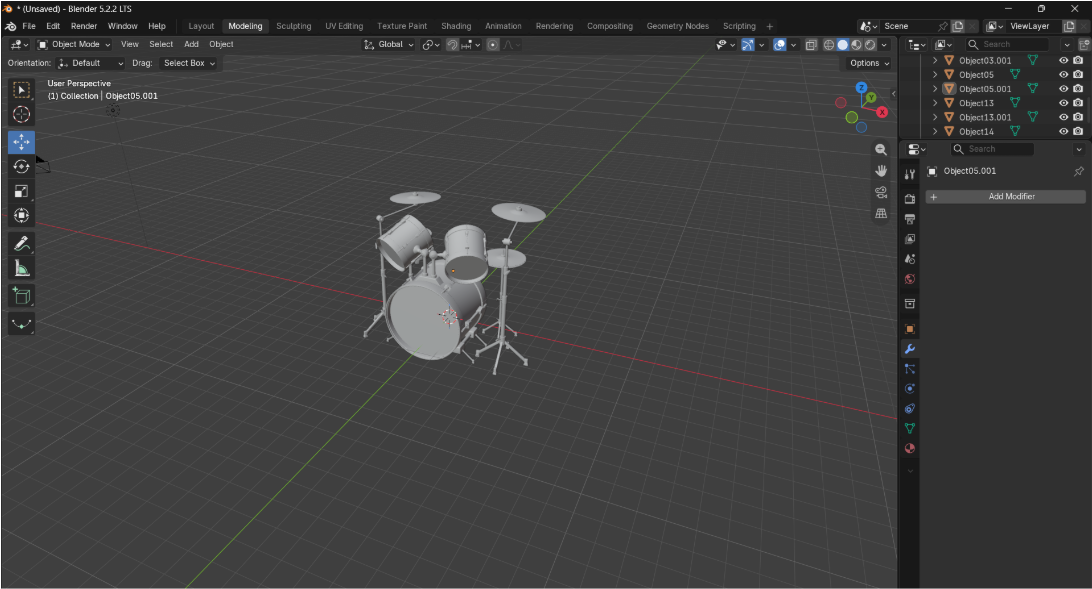
\includegraphics[width=0.62\linewidth]{bateria.png}
\caption{\label{fig:bateria}Imagen del \textit{asset} de batería en Blender para demostrar todos los componentes del instrumento.}
\end{figure}

\subsection{Evolución del prototipo (Baja a Alta Fidelidad) y navegación del usuario}
El prototipado de la interfaz y del entorno se realizó combinando la revisión del modelo 3D en Blender con herramientas de generación visual asistida por Inteligencia Artificial, abarcando desde su concepción estructural de baja fidelidad hasta un prototipo visual de alta fidelidad pensado para el visor \textbf{Meta Quest 2}:

\begin{itemize}
    \item \textbf{Prototipo de Baja Fidelidad (\textit{Wireframe}):} En una primera fase (Figura \ref{fig:baja_fidelidad}), se diseñó un esquema en escala de grises para definir el flujo de navegación: el ingreso al menú inicial con las dos opciones de batería (acústica y electrónica) y el ajuste de volumen, seguido de la vista en planta con el área de teletransportación frente a las siete piezas del instrumento. Este esquema resume el flujo general y es anterior a la incorporación del \textit{hi-hat}; en la Sección \ref{sec:escenas} se detalla cada escena por separado, con la distribución actualizada de ocho piezas.
\end{itemize}

\begin{figure}[H]
\centering
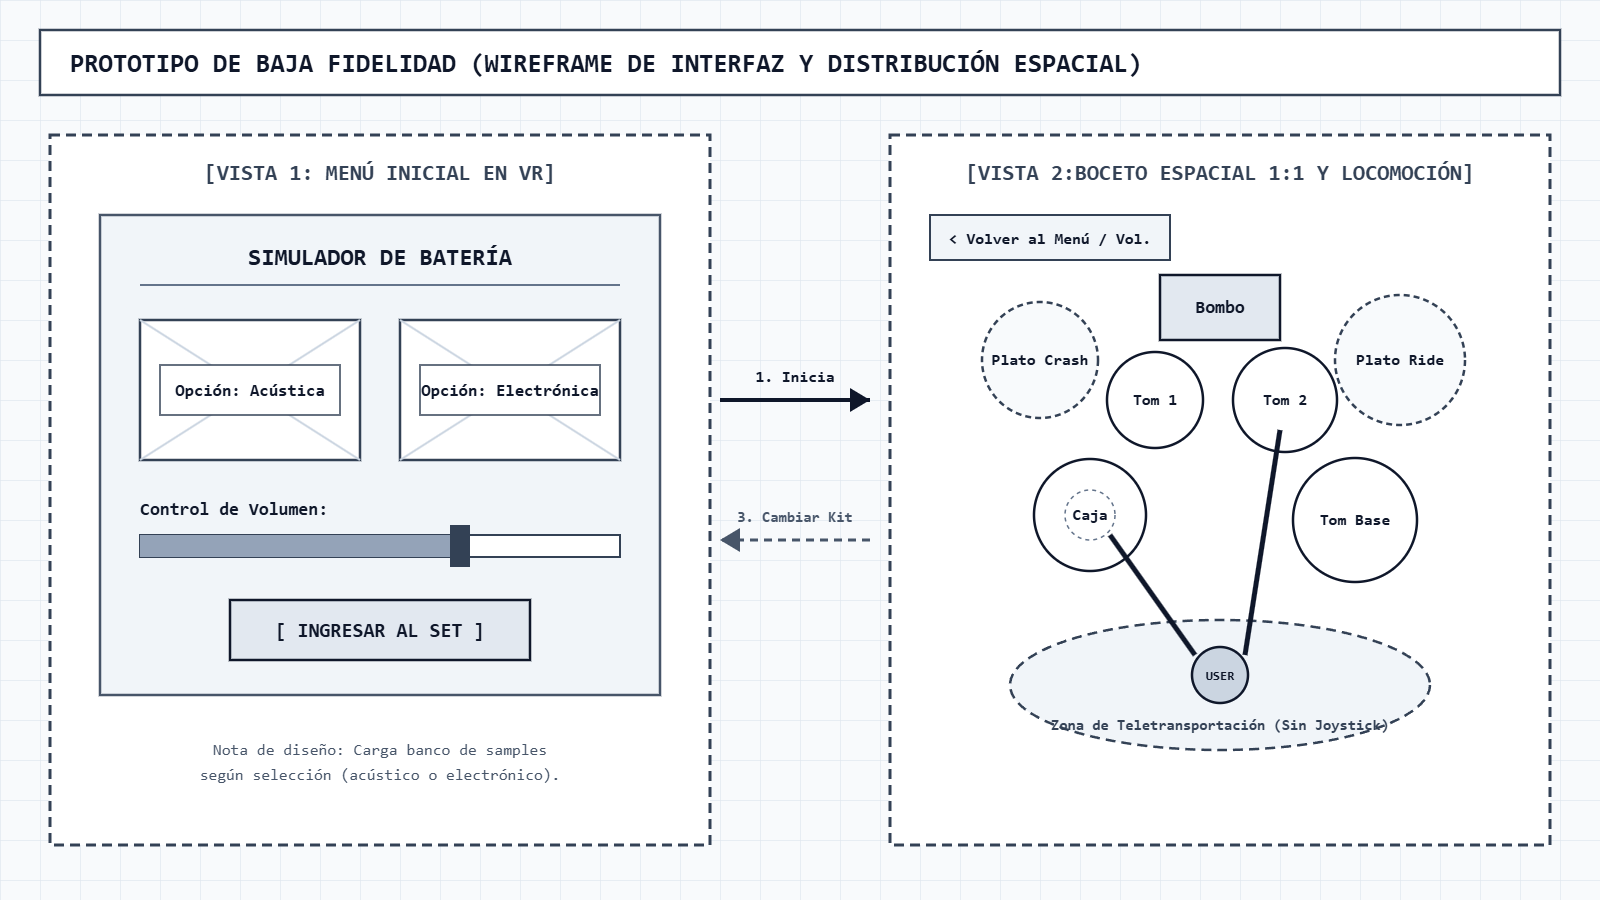
\includegraphics[width=0.82\linewidth]{baja_fidelidad.png}
\caption{\label{fig:baja_fidelidad}Prototipo de baja fidelidad (\textit{wireframe}) ilustrando el flujo entre el menú inicial y la distribución espacial con teletransportación.}
\end{figure}

\begin{itemize}
    \item \textbf{Prototipo de Alta Fidelidad y navegación en VR:} En la Figura \ref{fig:alta_fidelidad} se presenta el prototipo visual de alta fidelidad desde la perspectiva en primera persona del usuario utilizando los controles de Meta Quest 2. El flujo de navegación funciona de la siguiente manera:
    \begin{enumerate}
        \item Al ingresar a la aplicación, el usuario visualiza el menú de configuración donde elige inicialmente entre la opción de batería acústica o electrónica (cargando sus respectivos \textit{samples}) y regula el nivel de volumen mediante el control deslizable (por ejemplo, al $75\%$).
        \item Luego de eso, el usuario aparece cercano a la batería de su elección a escala real y tiene la capacidad de moverse por el mapa mediante \textbf{teletransportación}, acomodándose en la posición perfecta frente al kit sin necesidad de estar dándole ligeros toques continuos al \textit{joystick}.
        \item Durante la sesión, el usuario sostiene las baquetas virtuales con los mandos para golpear cada componente de la batería, pudiendo abrir nuevamente el panel flotante de configuración con el botón de menú del mando izquierdo si desea cambiar de kit de sonido o reajustar el volumen.
    \end{enumerate}
\end{itemize}

\begin{figure}[H]
\centering
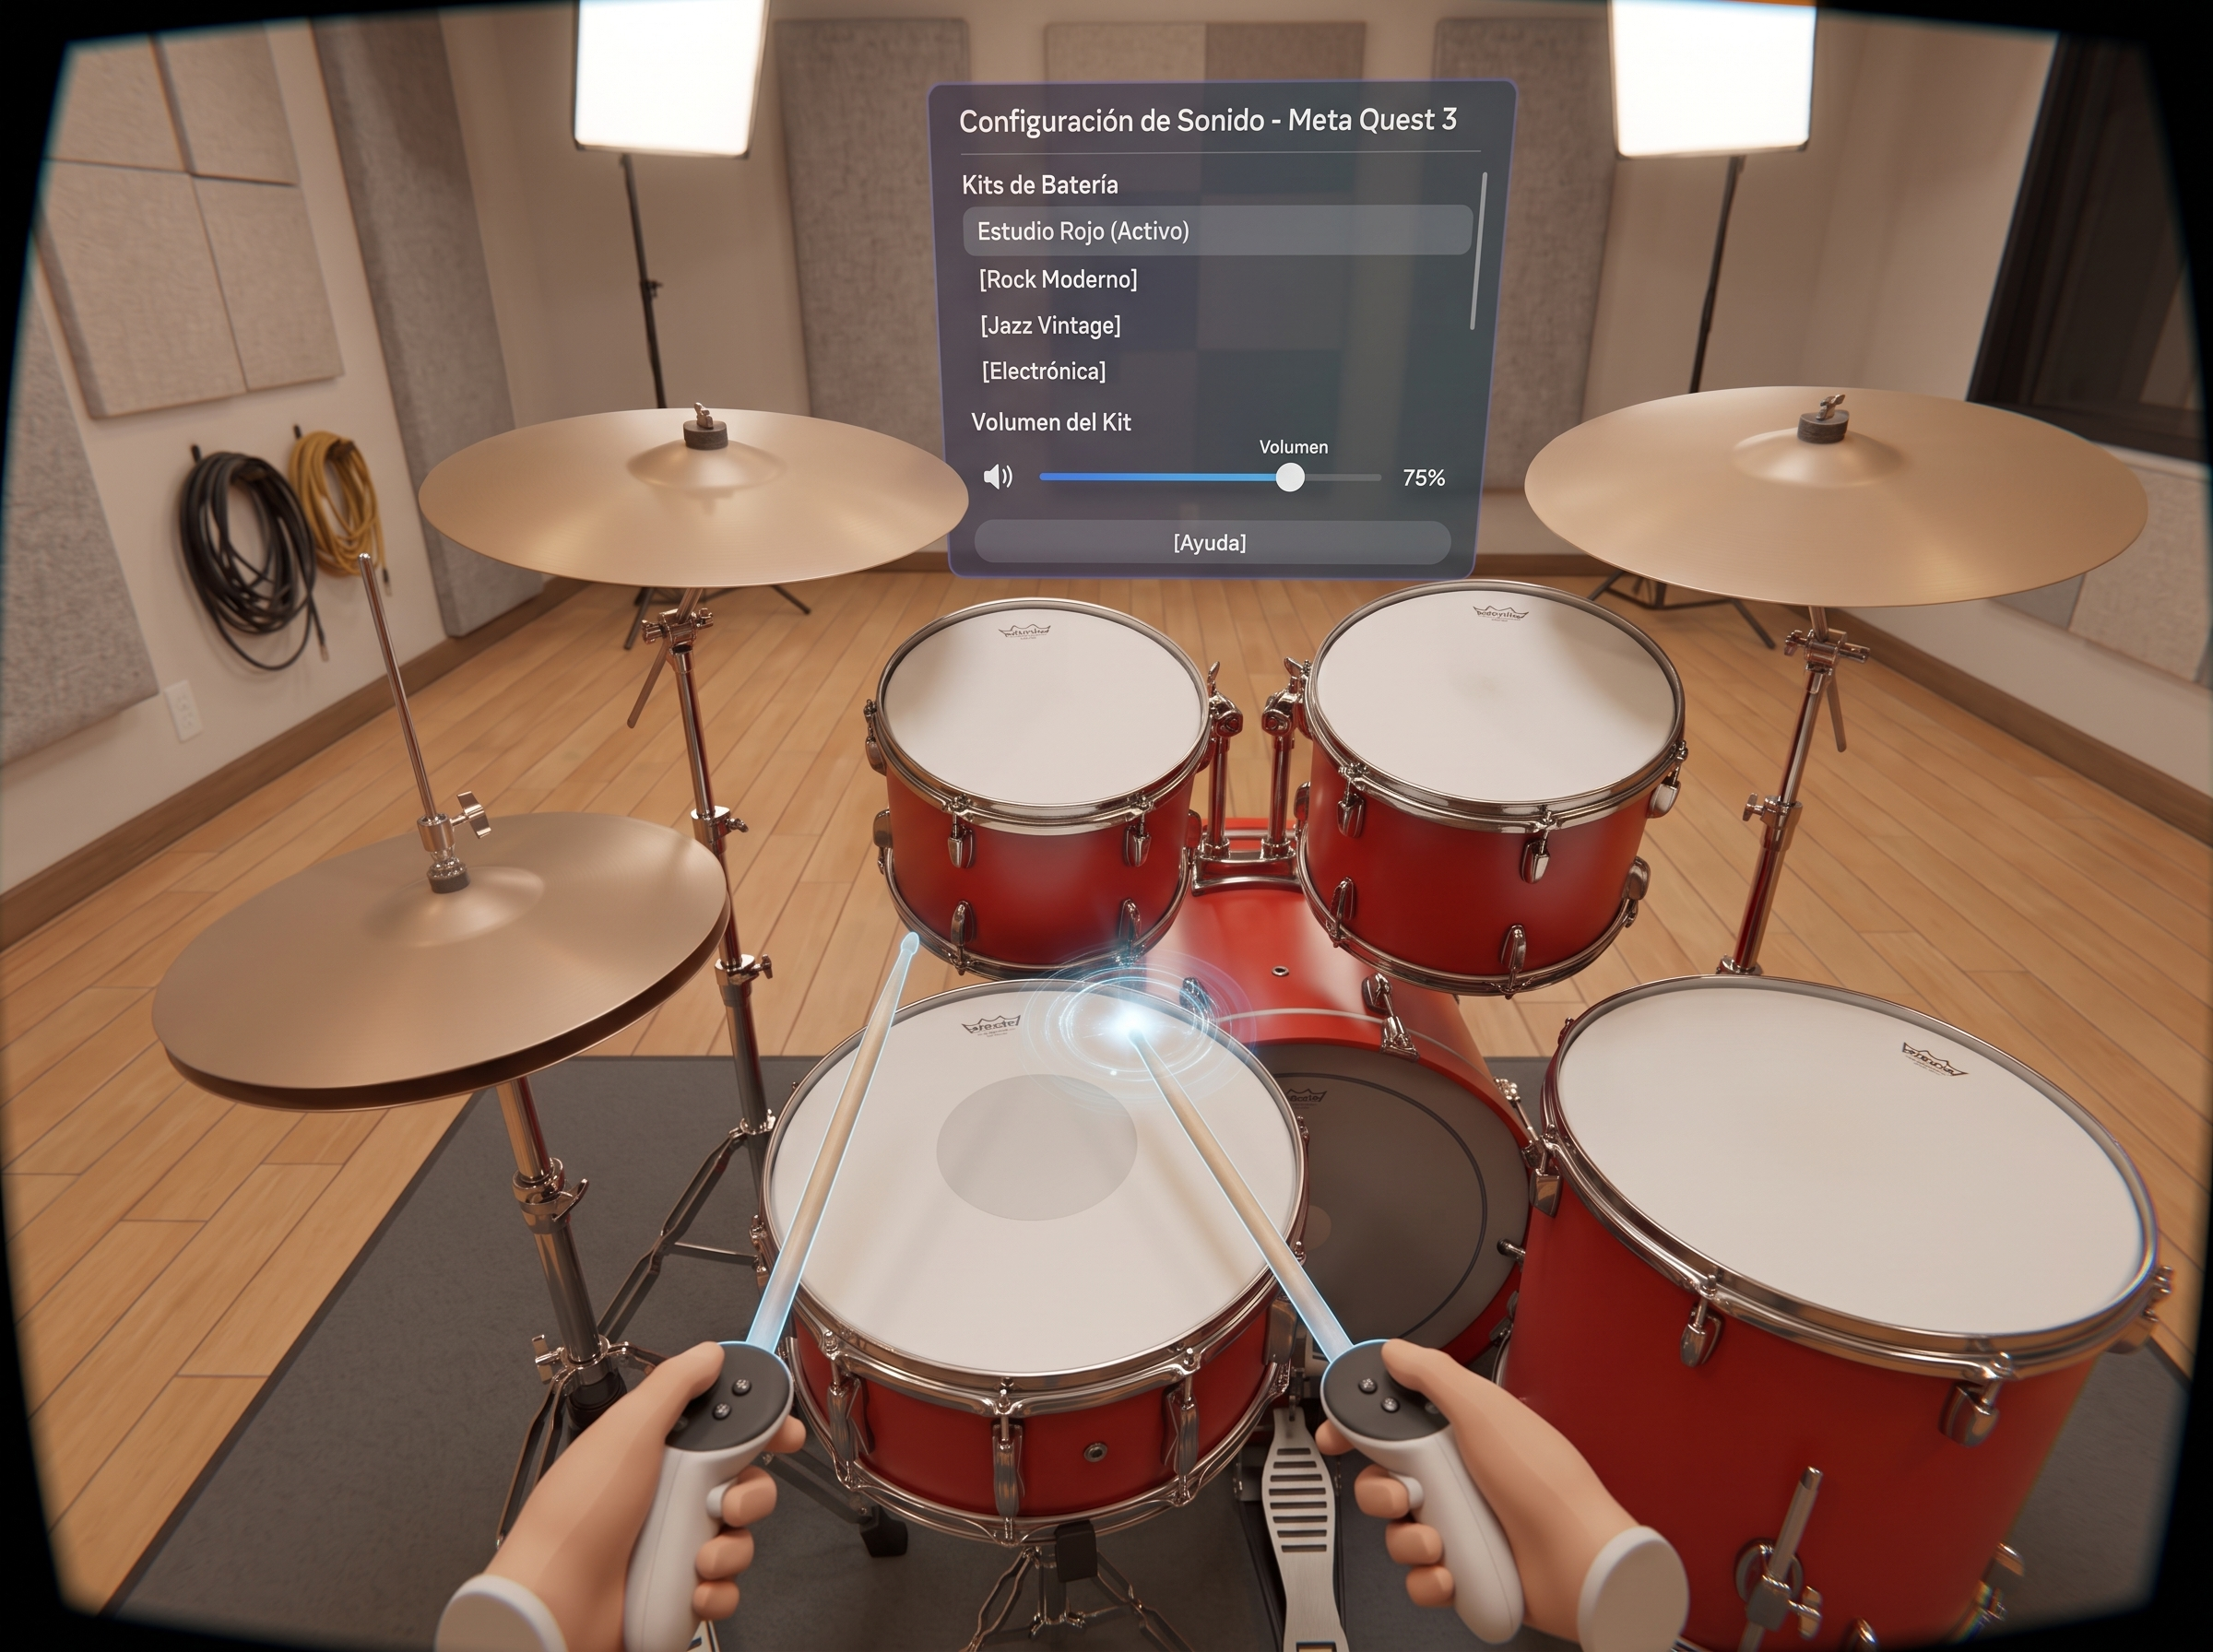
\includegraphics[width=0.6\linewidth]{alta_fidelidad_vr.jpg}
\caption{\label{fig:alta_fidelidad}Prototipo de alta fidelidad (generado con IA) mostrando la vista en primera persona en Meta Quest 2, el panel de configuración de sonido/volumen y la interacción de las baquetas con la batería.}
\end{figure}

\subsection{Detalle del prototipo por escena}
\label{sec:escenas}
La aplicación se divide en dos escenas de Unity. La primera es el menú inicial, donde el usuario configura su sesión, y la segunda es el estudio de práctica, donde está la batería. Lo que el usuario elige en el menú (tipo de batería y volumen) se guarda en un objeto que no se destruye al cambiar de escena (\texttt{DontDestroyOnLoad}), así el estudio se carga ya con el banco de \textit{samples} y el volumen correctos. Dentro del estudio también existe un panel de sesión, que no es una escena aparte sino un panel flotante que aparece sobre la escena 2 cuando el usuario lo llama. A continuación describimos cada escena por separado, y en el Cuadro \ref{tab:controles} resumimos qué hace cada control del Meta Quest 2 en cada una.

\subsubsection{Escena 1: Menú inicial}
Es lo primero que ve el usuario al abrir la aplicación. El entorno es una sala oscura y vacía con una luz suave sobre el panel, para que toda la atención vaya a la configuración. El panel es un \textit{Canvas} en espacio de mundo que aparece a unos $1.5$ m del usuario y centrado a la altura de sus ojos (Figura \ref{fig:escena1}). A esa distancia el texto se lee sin forzar la vista y el panel no se siente pegado a la cara.

\begin{figure}[H]
\centering
\begin{tikzpicture}[font=\sffamily\scriptsize, >=Stealth]
  % Vista frontal del panel
  \draw[black!70, fill=black!4, rounded corners=3pt] (0,0) rectangle (7,5.2);
  \node[font=\sffamily\bfseries\small] at (3.5,4.75) {DrumsAtHome VR};
  \draw[black!40] (0.5,4.4) -- (6.5,4.4);
  \node[anchor=west] at (0.5,4.1) {Elige tu batería:};
  % tarjeta acústica (seleccionada)
  \draw[black!85, line width=1.2pt, fill=white] (0.5,2.45) rectangle (3.3,3.85);
  \draw[black!30] (0.75,2.95) rectangle (3.05,3.7);
  \draw[black!30] (0.75,2.95) -- (3.05,3.7) (0.75,3.7) -- (3.05,2.95);
  \node at (1.9,2.7) {Batería acústica};
  % tarjeta electrónica
  \draw[black!60, fill=white] (3.7,2.45) rectangle (6.5,3.85);
  \draw[black!30] (3.95,2.95) rectangle (6.25,3.7);
  \draw[black!30] (3.95,2.95) -- (6.25,3.7) (3.95,3.7) -- (6.25,2.95);
  \node at (5.1,2.7) {Batería electrónica};
  \node[black!60, font=\sffamily\tiny] at (1.9,2.27) {(seleccionada por defecto)};
  % slider de volumen
  \node[anchor=west] at (0.5,1.85) {Volumen general};
  \draw[black!60, fill=white] (0.5,1.35) rectangle (5.7,1.55);
  \fill[black!45] (0.5,1.35) rectangle (4.4,1.55);
  \draw[black!85, fill=black!70] (4.3,1.25) rectangle (4.5,1.65);
  \node[anchor=west] at (5.85,1.45) {75\,\%};
  % botones
  \draw[black!80, fill=black!12] (0.5,0.35) rectangle (4.2,0.85);
  \node[font=\sffamily\scriptsize\bfseries] at (2.35,0.6) {Ingresar al estudio};
  \draw[black!60, fill=black!5] (4.6,0.35) rectangle (6.5,0.85);
  \node at (5.55,0.6) {Salir};
  \node[font=\sffamily\small] at (3.5,-0.45) {Vista frontal del panel};

  % Vista lateral
  \begin{scope}[xshift=8cm]
    \draw[black!50] (-0.2,0) -- (4.9,0);
    % usuario
    \draw[black!80, thick] (0.6,3.45) circle (0.25);
    \draw[black!80, thick] (0.6,3.2) -- (0.6,1.6);
    \draw[black!80, thick] (0.6,1.6) -- (0.35,0) (0.6,1.6) -- (0.85,0);
    \draw[black!80, thick] (0.6,2.8) -- (1.05,2.3);
    \draw[black!80, fill=black!30] (1.0,2.2) rectangle (1.2,2.4);
    % linea de los ojos y panel
    \draw[black!50, dashed] (0.85,3.45) -- (4.3,3.45);
    \draw[black!85, line width=2.5pt] (4.3,2.75) -- (4.3,4.15);
    \node[anchor=west, align=left] at (4.4,3.45) {Panel};
    % rayo del mando
    \draw[black!70, ->] (1.2,2.35) -- (4.25,3.05);
    \node[black!70, rotate=13] at (2.75,2.45) {rayo del mando};
    % cota
    \draw[<->, black!70] (0.6,-0.3) -- (4.3,-0.3);
    \node[fill=white, inner sep=1pt] at (2.45,-0.3) {$\approx 1.5$ m};
    \node[black!60, anchor=south] at (2.6,3.5) {altura de los ojos};
    \node[font=\sffamily\small] at (2.45,-0.8) {Vista lateral};
  \end{scope}
\end{tikzpicture}
\caption{\label{fig:escena1}Escena 1 (menú inicial). A la izquierda, el panel visto de frente; a la derecha, la distancia y la altura a la que aparece frente al usuario.}
\end{figure}

\begin{itemize}
    \item \textbf{Elementos:} el título de la aplicación, dos tarjetas para elegir el tipo de batería (acústica o electrónica), un \textit{slider} de volumen general de $0$ a $100\%$ que muestra el valor elegido, el botón \textit{Ingresar al estudio} y el botón \textit{Salir}. Para evitar errores, la batería acústica viene seleccionada por defecto y el volumen inicia en $75\%$, de modo que el botón de ingreso funciona aunque el usuario no cambie nada.
    \item \textbf{Interacción:} cada mando proyecta un rayo; el usuario apunta a una opción y presiona el gatillo para elegirla. El \textit{slider} se mueve apuntando a la perilla y arrastrándola con el gatillo presionado.
    \item \textbf{Retroalimentación:} al pasar el rayo sobre un botón este se resalta, y al presionarlo suena un clic y el mando vibra brevemente. Cuando se elige un tipo de batería se reproduce un golpe corto de caja con ese banco de \textit{samples}, y al soltar el \textit{slider} se repite el golpe con el volumen nuevo, para que el usuario pueda calibrarlo sin tener que entrar al estudio.
    \item \textbf{Transición:} al presionar \textit{Ingresar al estudio} la imagen se funde a negro durante medio segundo y se carga la escena 2. Usamos el fundido para que el cambio de entorno no sea brusco y no provoque mareo.
    \item \textbf{Requisitos que cubre:} RF1 y RF4.
\end{itemize}

\subsubsection{Escena 2: Estudio de práctica}
Es la escena principal, donde ocurre la práctica. Representa un cuarto de ensayo de unos $4 \times 3.2$ m con paneles acústicos en las paredes, una alfombra bajo la batería y una luz cálida enfocada en el kit, siguiendo el prototipo de alta fidelidad. La Figura \ref{fig:escena2} muestra la vista en planta con las ocho piezas a escala real, la banqueta, el punto donde aparece el usuario y la posición del panel de sesión.

\begin{figure}[H]
\centering
\begin{tikzpicture}[x=2.6cm, y=2.6cm, font=\sffamily\scriptsize, >=Stealth]
  % cuarto y piso teletransportable
  \draw[black!80, line width=1.2pt] (0,0) rectangle (4,3.2);
  \draw[black!40, dashed, fill=black!3] (0.12,0.12) rectangle (3.88,3.08);
  \node[black!60, anchor=north east] at (3.85,3.05) {Zona de teletransportación (todo el piso)};
  % alfombra
  \draw[black!35, fill=black!9] (0.85,0.85) rectangle (3.2,2.85);
  \node[black!55, anchor=south east] at (3.18,0.87) {Alfombra};
  % bombo (visto desde arriba)
  \draw[black!80, fill=white] (1.72,1.83) rectangle (2.28,2.28);
  \node at (2,2.055) {Bombo};
  % tambores
  \draw[black!80, fill=white] (1.58,1.60) circle (0.178);
  \node at (1.58,1.60) {Caja};
  \draw[black!80, fill=white] (1.82,2.48) circle (0.125);
  \node[font=\sffamily\tiny] at (1.82,2.48) {Tom 1};
  \draw[black!80, fill=white] (2.20,2.50) circle (0.15);
  \node[font=\sffamily\tiny] at (2.20,2.50) {Tom 2};
  \draw[black!80, fill=white] (2.55,1.55) circle (0.20);
  \node[font=\sffamily\tiny, align=center] at (2.55,1.55) {Tom\\base};
  % platos (más altos, borde punteado)
  \draw[black!80, dashed, fill=white] (1.35,2.45) circle (0.20);
  \node[font=\sffamily\tiny] at (1.35,2.45) {Crash};
  \draw[black!80, dashed, fill=white] (1.15,1.88) circle (0.178);
  \node[font=\sffamily\tiny] at (1.15,1.88) {Hi-hat};
  \draw[black!80, dashed, fill=white] (2.80,2.30) circle (0.255);
  \node[font=\sffamily\tiny] at (2.80,2.30) {Ride};
  % banqueta con ancla de teletransportación
  \draw[black!80, fill=black!20] (2,1.15) circle (0.18);
  \node[font=\sffamily\tiny] at (2,1.15) {Banqueta};
  \draw[->, thick, black!80] (2,1.36) -- (2,1.66);
  \draw[black!60] (2.14,1.04) -- (2.75,0.62);
  \node[anchor=north, align=center] at (2.75,0.6) {Ancla de teletransportación\\(deja al usuario mirando el kit)};
  % punto de aparición
  \draw[black!80, fill=white] (0.6,0.7) circle (0.1);
  \draw[->, black!80] (0.6,0.8) -- (0.6,0.98);
  \node[anchor=north, align=center] at (0.6,0.57) {Punto de\\aparición};
  \draw[->, black!60, dashed] (0.72,0.74) to[bend right=20] (1.8,1.08);
  \node[black!60, rotate=8] at (1.3,0.66) {teletransporte};
  % panel de sesión (visto desde arriba)
  \draw[black!85, line width=2.5pt] (0.7,1.1) -- (0.88,1.5);
  \node[anchor=south, align=center] at (0.42,1.56) {Panel de sesión\\(botón de menú)};
  % escala
  \draw[black!80, |-|] (3.0,-0.12) -- (4.0,-0.12);
  \node[anchor=north] at (3.5,-0.14) {1 m};
\end{tikzpicture}
\caption{\label{fig:escena2}Escena 2 (estudio de práctica) en vista de planta a escala. Los platos y el \textit{hi-hat} tienen borde punteado porque están a mayor altura que los tambores. La flecha sobre la banqueta indica hacia dónde queda mirando el usuario al teletransportarse.}
\end{figure}

\begin{itemize}
    \item \textbf{Elementos:} la batería de ocho piezas a escala 1:1 (RNF4) con la distribución de un kit para diestros: la caja a la izquierda de la banqueta, el \textit{hi-hat} a la izquierda de la caja, el bombo al centro, el \textit{Tom 1} y el \textit{Tom 2} sobre el bombo, el \textit{tom base} a la derecha, el plato \textit{crash} adelante a la izquierda y el \textit{ride} adelante a la derecha. Cada pieza tiene su propio \textit{collider}, su \texttt{AudioSource} y un script que conoce su centro y su radio para calcular la zona de impacto. Las dos baquetas aparecen apoyadas sobre la caja.
    \item \textbf{Llegada y locomoción:} el usuario aparece de pie a un costado del kit, como se ve en la Figura \ref{fig:escena2}. Sobre la banqueta hay un ancla de teletransportación que, además de moverlo, lo deja mirando hacia la batería, así no tiene que girar ni corregir su posición a mano. El resto del piso es una zona de teletransportación libre por si quiere ver el kit desde otro lugar. El arco de teletransportación solo aparece mientras el \textit{joystick} se mantiene inclinado hacia adelante, para que un roce del pulgar mientras toca no lo mueva de sitio.
    \item \textbf{Interacción con la batería:} el usuario acerca la mano a una baqueta y presiona una vez el botón de agarre (\textit{grip}) para tomarla; la baqueta se queda en la mano hasta que lo vuelva a presionar. Decidimos que no haya que mantener el botón apretado porque en una sesión larga eso cansa la mano. Con las baquetas golpea el \textit{hi-hat}, los platos, los \textit{toms} y la caja. Los gatillos quedan libres bajo los dedos índice mientras se sujetan las baquetas, así que los usamos como pedales: el derecho toca el bombo y el izquierdo cierra el \textit{hi-hat}. Si el gatillo izquierdo está suelto, el \textit{hi-hat} suena abierto; presionado a medias, semiabierto; y presionado del todo, cerrado. Presionarlo de golpe sin usar la baqueta hace sonar el choque de los dos platos al cerrarse, como cuando se pisa el pedal.
    \item \textbf{Retroalimentación:} cada golpe reproduce el \textit{sample} de la pieza con un volumen según la velocidad y un tono según la zona (RF3), el mando vibra brevemente con una intensidad proporcional a la fuerza y, en el caso de los platos, el plato golpeado se balancea un poco. Además, el plato superior del \textit{hi-hat} sube o baja siguiendo el gatillo izquierdo, para que el usuario vea si está abierto o cerrado sin tener que deducirlo por el sonido.
    \item \textbf{Panel de sesión:} al presionar el botón de menú del mando izquierdo aparece un panel flotante a la izquierda del usuario, para no tapar la batería, con las mismas opciones del menú inicial (tipo de batería y volumen) y los botones \textit{Volver al menú} y \textit{Salir}. Mientras el panel está abierto, los mandos vuelven a mostrar el rayo y los gatillos dejan de funcionar como pedales para servir como selección. Cambiar de batería desde aquí no recarga la escena: solo se reemplaza el banco de \textit{samples}, y el usuario sigue en el mismo lugar.
    \item \textbf{Transición:} \textit{Volver al menú} hace el mismo fundido a negro y carga la escena 1 con la configuración actual ya marcada.
    \item \textbf{Requisitos que cubre:} RF2, RF3, RF5, RNF1, RNF2, RNF3 y RNF4, además de RF1 y RF4 a través del panel de sesión.
\end{itemize}

\begin{table}[H]
\centering
\small
\renewcommand{\arraystretch}{1.35}
\begin{tabular}{@{} >{\raggedright\arraybackslash}p{0.24\textwidth} >{\raggedright\arraybackslash}p{0.30\textwidth} >{\raggedright\arraybackslash}p{0.38\textwidth} @{}}
\toprule
\textbf{Control del Meta Quest 2} & \textbf{Escena 1: Menú inicial} & \textbf{Escena 2: Estudio de práctica} \\
\midrule
Gatillo derecho & Seleccionar con el rayo y arrastrar el \textit{slider}. & Tocar el bombo. Con el panel de sesión abierto, seleccionar opciones. \\
Gatillo izquierdo & Seleccionar con el rayo y arrastrar el \textit{slider}. & Pedal del \textit{hi-hat}: suelto queda abierto, a medias semiabierto y presionado cerrado. Con el panel de sesión abierto, seleccionar opciones. \\
Botón de agarre (\textit{grip}) & Sin uso. & Un toque toma la baqueta y otro toque la suelta. \\
\textit{Joystick} & Sin uso. & Inclinado hacia adelante muestra el arco de teletransportación; al soltarlo, el usuario se mueve al punto marcado. \\
Botón de menú (mando izquierdo) & Sin uso. & Abre y cierra el panel de sesión. \\
Botón Meta (mando derecho) & Reservado por el sistema. & Reservado por el sistema. \\
\bottomrule
\end{tabular}
\caption{\label{tab:controles}Acciones asignadas a cada control del Meta Quest 2 en cada escena.}
\end{table}

\subsection{Propuesta de implementación técnica, decisiones de diseño y usabilidad}
Si bien en este primer hito el prototipo se elaboró a nivel visual y conceptual con apoyo de IA y Blender, para su futura implementación funcional se ha proyectado utilizar el motor \textbf{Unity} y el lenguaje de programación \textbf{C\#}, con OpenXR y el paquete XR Interaction Toolkit para el visor \textbf{Meta Quest 2}, que es el que tenemos disponible en el curso. La elección de estas herramientas responde a la necesidad de manipular directamente las físicas y el audio para resolver nuestra problemática técnica principal: como la batería en muchas canciones exige una interacción muy rápida y fuerte, tendríamos problemas con el refrescado y la detección de frames, además del riesgo de que las baquetas atraviesen las baterías, lo cual nunca debe ocurrir.

La manera en la que pensamos afrontar esta problemática durante el desarrollo se basa en cuatro posibles mecanismos (esquematizados en la Figura \ref{fig:fisicas_vr}):

\begin{enumerate}
    \item \textbf{Colisión continua y \textit{Sweep Test}:} A través de usar \textit{Continuous Collision Detection} (CCD), usaremos \texttt{Rigidbody} en nuestras baquetas para que constantemente colisionen con lo que interactúen, en este caso con la batería. También se usará \textit{Raycast/Sweep Test} junto con CCD: las baquetas crearán un hitbox (\texttt{Physics.SphereCast}) desde la posición del frame anterior hacia la posición actual para saber que están interactuando con la batería sin atravesarla. Para dimensionar el problema: si la punta de la baqueta baja a unos $5$ m/s y la física de Unity se actualiza cada $0.02$ s (su valor por defecto), entre un paso y el siguiente la punta avanza $10$ cm, mucho más que el grosor del \textit{collider} de un parche. Por eso también igualaremos el \textit{Fixed Timestep} a la frecuencia del Meta Quest 2 ($1/72$ s); aun así la punta avanzaría unos $7$ cm por paso, lo que confirma que el CCD y el barrido siguen siendo necesarios.
    \item \textbf{Cálculo manual de velocidad:} Para calcular la velocidad no se usará la velocidad de \texttt{Rigidbody}, ya que el seguimiento de VR no es $100\%$ confiable. Por ello, deberemos calcular manualmente la velocidad de los controles con un \textit{buffer} de entre $3$ a $5$ frames. La velocidad será la posición actual menos la posición guardada $n$ frames atrás, dividida entre el tiempo que pasó entre esos dos frames:
    \[
    \vec{v} = \frac{\vec{P}_{k} - \vec{P}_{k-n}}{t_{k} - t_{k-n}}, \quad 3 \le n \le 5
    \]
    donde $k$ es el frame actual. Al usar varios frames en lugar de solo el anterior, un error de posición en un frame aislado se divide entre un intervalo de tiempo mayor y pesa menos en el resultado.
    \item \textbf{Cálculo de zona o distancia de impacto:} Para calcular la distancia o zona de la batería que fue golpeada por las baquetas, se convertirá la colisión \texttt{ContactPoint.point} al espacio local del objeto batería. Se calculará el radio como la distancia entre el contacto local y el centro, dividida entre el radio de la batería, tomando valores entre $0.0$ (el centro) y $1.0$ (el borde):
    \[
    r = \frac{\text{distancia}(\text{Contacto}_{\text{local}}, \text{Centro})}{\text{Radio de la batería}}, \quad r \in [0.0, 1.0]
    \]
    \item \textbf{Mecánicas de audio dinámicas:} Se usará \texttt{AudioSource.pitch} y se ajustará el volumen para producir el efecto de fuerza y zona con el que se golpeó el componente de la batería. En el \textit{hi-hat} se usarán dos muestras, cerrado y abierto, y la apertura intermedia se obtendrá mezclando ambas según el valor del gatillo izquierdo al momento del golpe. Si el usuario cierra el \textit{hi-hat} mientras todavía suena abierto, ese sonido se corta, como ocurre en una batería real.
\end{enumerate}

\begin{figure}[H]
\centering
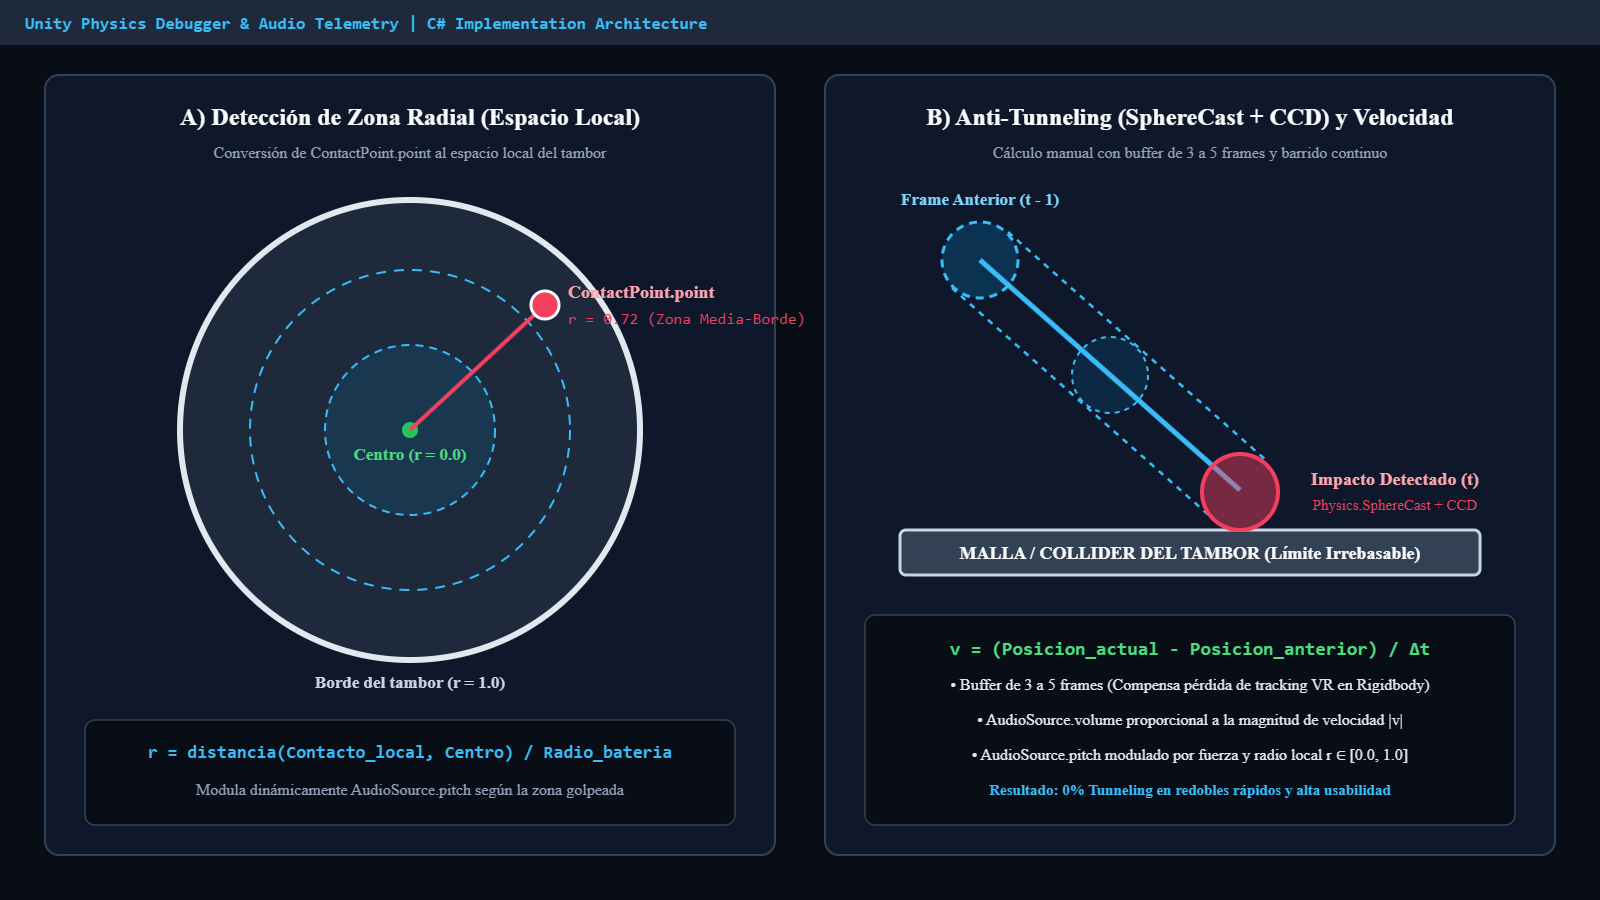
\includegraphics[width=0.82\linewidth]{fisicas_vr.png}
\caption{\label{fig:fisicas_vr}Esquema técnico de la lógica de implementación proyectada para la zona radial ($0.0$ a $1.0$) y la prevención de atravesamiento mediante \texttt{Physics.SphereCast} y \textit{buffer} de frames.}
\end{figure}

\textbf{Impacto de los retos de implementación en la usabilidad de la interfaz:}
Planificar estas decisiones técnicas desde el diseño es fundamental para no comprometer la usabilidad de la interfaz. Si durante la implementación no se corrigieran las limitaciones de detección de frames mediante CCD y \texttt{Physics.SphereCast}, los golpes rápidos no emitirían sonido y las baquetas atravesarían los tambores, generando frustración y rompiendo la inmersión del usuario. De igual manera, calcular la velocidad con un \textit{buffer} manual evita volúmenes erráticos causados por pérdidas momentáneas de seguimiento en los controles VR, mientras que la locomoción por teletransportación asegura una navegación cómoda y libre de mareos.

\section{Cronograma en formato Gantt}

Para organizar la implementación de los requerimientos planteados en este informe, se ha estructurado el cronograma de trabajo distribuido entre las Semanas 10 y 15 del semestre académico. En el Cuadro \ref{tab:gantt} se presenta el diagrama de Gantt con la planificación progresiva de los entregables (del $15\%$ al $100\%$) y la presentación final; la tercera columna indica qué requisitos funcionales y no funcionales se implementan en cada entregable.

\begin{table}[H]
\centering
\small
\setlength{\tabcolsep}{4pt}
\renewcommand{\arraystretch}{1.45}
\begin{tabular}{@{} >{\bfseries\raggedright\arraybackslash}p{0.15\textwidth} >{\raggedright\arraybackslash}p{0.33\textwidth} >{\raggedright\arraybackslash}p{0.11\textwidth} c c c c c c @{}}
\toprule
Entregable & \textbf{Actividades} & \textbf{RF/RNF} & \textbf{S10} & \textbf{S11} & \textbf{S12} & \textbf{S13} & \textbf{S14} & \textbf{S15} \\
\midrule
Entregable 1 \newline \normalfont\footnotesize(15\% - Sem. 10) &
Escena 2 base: cuarto de ensayo, integración del \textit{asset} 3D de la batería (ocho piezas, con \textit{hi-hat}) y las baquetas a escala real, y teletransportación con ancla en la banqueta. Escena 1 creada con sus botones, todavía sin cargar \textit{samples}. &
RF5, RNF4, RF1 (parcial) &
\rule{0.45cm}{0.28cm} & & & & & \\
\addlinespace[0.3em]

Entregable 2 \newline \normalfont\footnotesize(30\% - Sem. 11) &
Menú inicial completo: selección de batería acústica o electrónica, \textit{slider} de volumen, paso de la configuración a la escena 2 y panel de sesión con el botón de menú. &
RF1, RF4 &
& \rule{0.45cm}{0.28cm} & & & & \\
\addlinespace[0.3em]

Entregable 3 \newline \normalfont\footnotesize(50\% - Sem. 12) &
Baquetas con agarre por toque, \texttt{Rigidbody} con \textit{Continuous Collision Detection} (CCD), barrido con \texttt{Physics.SphereCast} entre frames, bombo con el gatillo derecho y pedal del \textit{hi-hat} con el gatillo izquierdo. &
RF2, RNF1 &
& & \rule{0.45cm}{0.28cm} & & & \\
\addlinespace[0.3em]

Entregable 4 \newline \normalfont\footnotesize(70\% - Sem. 13) &
Cálculo de velocidad con \textit{buffer} de $3$ a $5$ frames y detección de la zona golpeada con \texttt{ContactPoint.point} en espacio local ($0.0$ centro a $1.0$ borde). &
RF3 (cálculo), RNF2 &
& & & \rule{0.45cm}{0.28cm} & & \\
\addlinespace[0.3em]

Entregable 5 \newline \normalfont\footnotesize(100\% - Sem. 14) &
Bancos de \textit{samples} acústico y electrónico, volumen y \texttt{AudioSource.pitch} según fuerza y zona, mezcla de \textit{hi-hat} abierto y cerrado, vibración del mando, medición de latencia y pruebas integrales. &
RF3 (audio), RNF3 &
& & & & \rule{0.45cm}{0.28cm} & \\
\addlinespace[0.3em]

Entregable 6 \newline \normalfont\footnotesize(Presentación - S15) &
Evaluación con usuarios, análisis de las métricas HEART, documentación del Hito 2 y presentación final del proyecto. &
Validación de todos &
& & & & & \rule{0.45cm}{0.28cm} \\
\bottomrule
\end{tabular}
\caption{\label{tab:gantt}Cronograma de trabajo en formato Gantt con los requisitos asignados a cada entregable (Semanas 10 a 15).}
\end{table}

Con esta distribución todos los requisitos quedan asignados a un entregable. RF1 y RF3 se reparten en dos porque dependen de partes que se construyen en momentos distintos: la escena del menú existe desde el Entregable 1, pero recién en el 2 carga los \textit{samples}; y el cálculo de fuerza y zona del RF3 se hace en el Entregable 4, antes de conectarlo con el audio en el 5. RNF3 queda en el Entregable 5 porque la latencia del sonido solo se puede medir cuando el audio ya está integrado.

\begin{thebibliography}{9}
\bibitem{batery_asset}
Free3D. \href{https://free3d.com/3d-model/drum-set-99664.html}{\textit{Drum Set 3D Model (Asset de la batería a usar)}}. Contiene la batería con cada pieza y baquetas con sus texturas respectivas.

\bibitem{samples}
Reddit Drumkits Community. \href{https://www.reddit.com/r/Drumkits/comments/y3vqbf/every_drum_machine_since_the_1970s/}{\textit{Samples de sonido para la batería}}. Repositorio de muestras de audio para las variantes acústica y electrónica de la batería.

\bibitem{glisson2023}
Glisson, M. (2023). \href{https://csbapp.uncw.edu/mscsisProceedings/2023/GlissonMorgan.pdf}{\textit{Utilizing Virtual Reality to Teach Drum Rudiments}}. University of North Carolina Wilmington.

\bibitem{paradiddle}
Tanirgan, E. (2023). \href{https://paradiddleapp.com/}{\textit{Paradiddle: Drumming Reimagined for Virtual Reality}}. Aplicación comercial de simulación de percusión en VR.
\end{thebibliography}

\end{document}
